%%% LaTeX Template: Designer's CV
%%%
%%% Source: http://www.howtotex.com/
%%% Feel free to distribute this template, but please keep the referal to HowToTeX.com.
%%% Date: March 2012


%%%%%%%%%%%%%%%%%%%%%%%%%%%%%%%%%%%%%
% Document properties and packages
%%%%%%%%%%%%%%%%%%%%%%%%%%%%%%%%%%%%%
\documentclass[a4paper,12pt,final]{memoir}

% misc
\renewcommand{\familydefault}{bch}	% font
\pagestyle{empty}					% no pagenumbering
\setlength{\parindent}{0pt}			% no paragraph indentation


% required packages (add your own)
\usepackage{flowfram}										% column layout
\usepackage[top=1cm,left=1cm,right=1cm,bottom=1cm]{geometry}% margins
\usepackage{graphicx}										% figures
\usepackage{url}											% URLs
\usepackage[usenames,dvipsnames]{xcolor}					% color
\usepackage{multicol}										% columns env.
	\setlength{\multicolsep}{0pt}
\usepackage{paralist}										% compact lists
\usepackage{tikz}

%%%%%%%%%%%%%%%%%%%%%%%%%%%%%%%%%%%%%
% Create column layout
%%%%%%%%%%%%%%%%%%%%%%%%%%%%%%%%%%%%%
% define length commands
\setlength{\vcolumnsep}{\baselineskip}
\setlength{\columnsep}{\vcolumnsep}

% frame setup (flowfram package)
% left frame
\newflowframe{0.2\textwidth}{\textheight}{0pt}{0pt}[left]
	\newlength{\LeftMainSep}
	\setlength{\LeftMainSep}{0.2\textwidth}
	\addtolength{\LeftMainSep}{1\columnsep}
 
% small static frame for the vertical line
\newstaticframe{1.5pt}{\textheight}{\LeftMainSep}{0pt}
 
% content of the static frame
\begin{staticcontents}{1}
\hfill
\tikz{%
	\draw[loosely dotted,color=RoyalBlue,line width=1.5pt,yshift=0]
	(0,0) -- (0,\textheight);}%
\hfill\mbox{}
\end{staticcontents}
 
% right frame
\addtolength{\LeftMainSep}{1.5pt}
\addtolength{\LeftMainSep}{1\columnsep}
\newflowframe{0.7\textwidth}{\textheight}{\LeftMainSep}{0pt}[main01]


%%%%%%%%%%%%%%%%%%%%%%%%%%%%%%%%%%%%%
% define macros (for convience)
%%%%%%%%%%%%%%%%%%%%%%%%%%%%%%%%%%%%%
\newcommand{\Sep}{\vspace{1.5em}}
\newcommand{\SmallSep}{\vspace{0.5em}}

\newenvironment{AboutMe}
	{\ignorespaces\textbf{\color{RoyalBlue} About me}}
	{\Sep\ignorespacesafterend}
	
\newcommand{\CVSection}[1]
	{\Large\textbf{#1}\par
	\SmallSep\normalsize\normalfont}

\newcommand{\CVItem}[1]
	{\textbf{\color{RoyalBlue} #1}}


%%%%%%%%%%%%%%%%%%%%%%%%%%%%%%%%%%%%%
% Begin document
%%%%%%%%%%%%%%%%%%%%%%%%%%%%%%%%%%%%%
\begin{document}

% Left frame
%%%%%%%%%%%%%%%%%%%%
\begin{figure}
	\hfill
	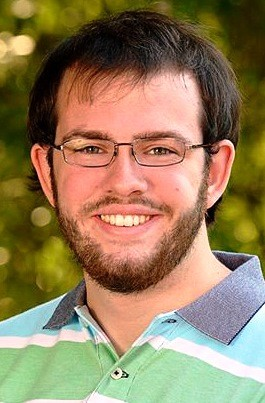
\includegraphics[width=0.75\columnwidth]{photo.png}
	\vspace{-7cm}
\end{figure}

\begin{flushright}\small
	Wesley Rogers \\
	***REMOVED*** \\
	***REMOVED*** \\
	***REMOVED*** \\
	\Sep
	\textbf{Mailing Address} \\
	Wesley Rogers \\
	Western Carolina University \\
	***REMOVED***\\
	***REMOVED*** \\
	***REMOVED*** \\
\end{flushright}\normalsize
\framebreak


% Right frame
%%%%%%%%%%%%%%%%%%%%
\Huge\bfseries {\color{RoyalBlue} Wesley Rogers} \\
%\Large\bfseries  Student \\
\normalsize\normalfont
% About me
%\begin{AboutMe}
%I’m an avid problem solver and student, and am currently an
%honors freshman at Western Carolina University. Currently, I am declared
%as a Traditional Mathematics and Computer Science double major. I have over a year of
%experience in Java, and a good amount in the Bash Shell script. I tend to
%learn new software very quickly, and have a large amount of linux and Java
% IDE experience. In addition, I also have basic skills in HTML, CSS, and %JavaScript.
%\end{AboutMe}

% Experience
\CVSection{Education}
\CVItem{August 2016 - present, \textit{Western Carolina University}}\\
{\color{RoyalBlue}$\circ$} Major: Computer Science \\
{\color{RoyalBlue}$\circ$} Major: Mathematics with Data Science concentration \\
{\color{RoyalBlue}$\circ$} GPA: 3.77 \\
{\color{RoyalBlue}$\circ$} Honors College Member \\

\CVSection{Experience}
\CVItem{Current, Lab Assistant/Tutor, \textit{WCU Computer Science and Math Dept.}}
Assisted in lab and tutored for the Introduction to Programming/Problem Solving I/II courses of the WCU CS Department, and as a math tutor at the WCU Math Tutoring Center.
\SmallSep

\CVItem{Summer 2018 \& 2019, Technical Intern, \textit{SAS Software}}\\
Worked as a technical intern under Eric Bourn to improve the efficiency and portability of the SAS Viya Mid-Tier Platform.
\Sep


\CVSection{Extracurriculars}
\CVItem{ACM Chapter President, \textit{Western Carolina University Chapter}}\\
Led the Western Carolina Chapter of the ACM for the 2017-2018 and 2018-2019 Academic Years, including multiple events.
\SmallSep

\CVItem{WCU Math Club Web Developer, \textit{Western Carolina University}}\\
Produced a small website for club activities, and helped run the club.

\Sep

\CVSection{Awards}
\CVItem{Fall 2016/Fall 2017 Chancellors' List, \textit{Western Carolina University}}\\
Chancellors' list designation, awarded to any student with a 3.8 or higher semester GPA.

\SmallSep

\CVItem{Spring 2017, Deans' List, \textit{Western Carolina University}}\\
Deans' list designation, awarded to any student with a 3.5 or higher semester GPA.

\SmallSep

\CVItem{Freshman Mathematics Award, \textit{Western Carolina University}}\\
Awarded for outstanding academic achievements in mathematics in the first year as an undergraduate student. Awarded in the Fall 2016-Spring 2017 academic year.

\Sep

% Skills
\CVSection{Computer Skills}
\CVItem{Programming}
\begin{multicols}{3}
	\begin{compactitem}[\color{RoyalBlue}$\circ$]
		\item Java
		\item Bash Shell
		\item C
		\item Python \& SciPy
		\item Rust
		\item Assorted Others
	\end{compactitem}
\end{multicols}
\SmallSep

\CVItem{Computer Software}
\begin{multicols}{3}
	\begin{compactitem}[\color{RoyalBlue}$\circ$]
		\item IntelliJ
		\item Linux Shell
		\item Mathematica
		\item LaTeX
		\item Excel
		\item SAS (Certified)
	\end{compactitem}
\end{multicols}



%%%%%%%%%%%%%%%%%%%%%%%%%%%%%%%%%%%%%
% End document
%%%%%%%%%%%%%%%%%%%%%%%%%%%%%%%%%%%%%
\end{document}
